Sprinkler-pumpe systemet består af en Hunter PS Pop-up sprinkler og en Alpha2 pumpe fra Grundfos, disse forbindes med passende slanger og fittings. For at styre sprinkleren, skal Alpha2 pumpen kunne tændes og afbrydes. Dette gøres via et 230 V / 5 V relæ. Dette relæ styres via én pin på Enheden. 


\subsection{230 V / 5 V relæ}

For at 230 V / 5 V relæet kan blive en realitet, er det pålagt, at dette bygges i en lukket kasse og godkendes af en elektronikværksteds-ansvarlig. Kassen som bygges har et 230 VAC apparat stik ind og en 230 VAC stikkontakt ud. For at skabe forbindelse/afbrydelse af denne 230 VAC strøm benyttes et relæ, dette relæ styres af 5 V. Når 5 V  tilføjes relæets spole, klikker relæet og der skabes gennemgang fra apparatstik til stikkontakt. Dette lukkede kredsløb bygges som tidligere nævnt, ind i en lukket kasse med gennemsigtigt låg. Relæet der benyttes er et Finder 40.52s. Figur \ref{lab:RELAY} viser kredsløbet for dette lukkede kredsløb.

\begin{figure}[H] \centering
{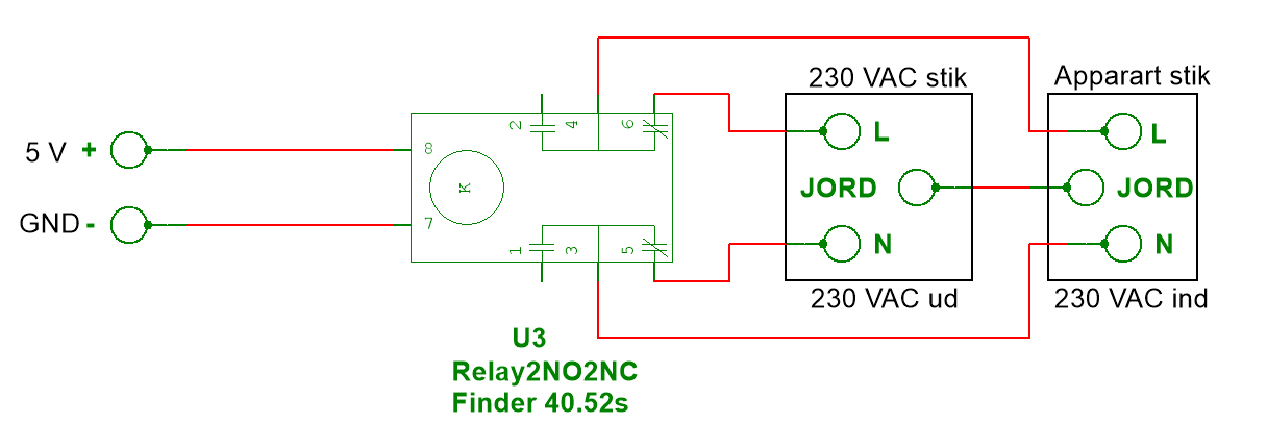
\includegraphics[width=\textwidth]{filer/design/Billeder/230VAC_KREDS}}
\caption{230 V / 5 V relæ}
\label{lab:RELAY}
\raggedright
\end{figure}

\subsection{Alpha2 pumpen}

Alpha2 pumpen skal blot tilsluttes 230 VAC + jord. Der medfølger et special stik til selve pumpen, dette forbindes til en 230 V stikprop, med 3-ledet kabel (Fase, Nul og Jord) . Stikproppen kan nu sættes i 230 V / 5 V relæets 230 V stikkontakt.

\begin{figure}[H] \centering
{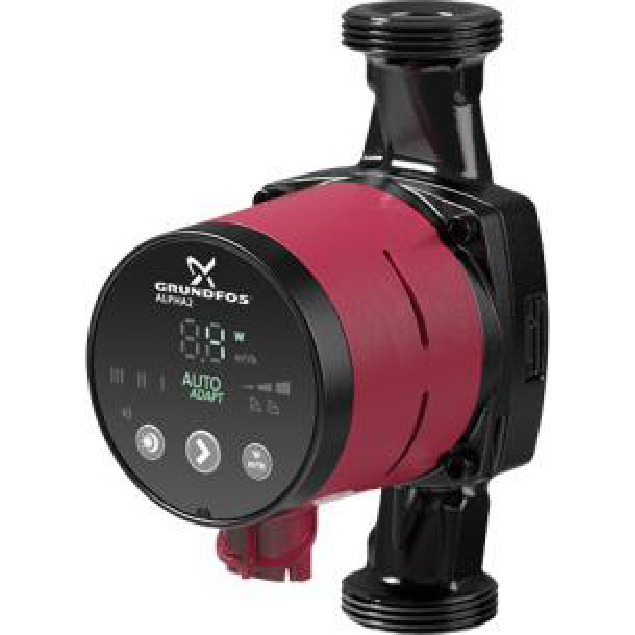
\includegraphics[width=0.4\textwidth]{filer/design/Billeder/Alpha2}}
\caption{Alpha2 Cirkulationspumpe fra Grundfos}
\label{lab:Alpha2}
\raggedright
\end{figure} 

\subsection{Relæstyring}

Ifølge databladet for Finder 40.52s (figur \ref{lab:finder4052s}), kræver relæet 100 mA ved 5 V forsyning.

\begin{figure}[H] \centering
{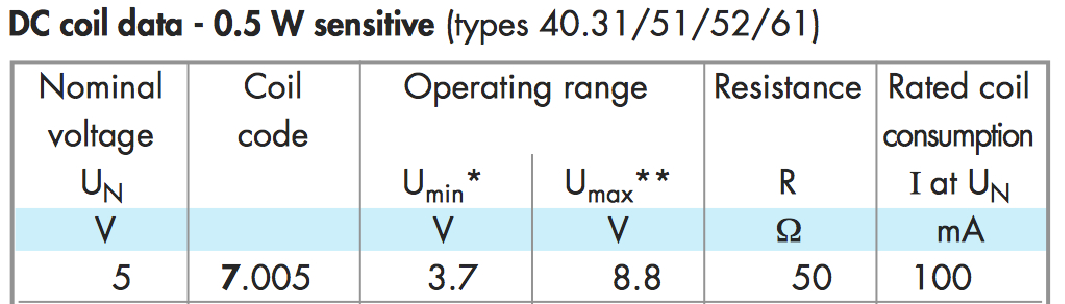
\includegraphics[width=0.7\textwidth]{filer/design/Billeder/finder4052s}}
\caption{Datablad for Finder 40.52s - 100 mA, side 7}
\label{lab:finder4052s}
\raggedright
\end{figure} 

PSoC'ens udgang giver hverken strøm eller spænding nok til at trække relæet. PSoC4 afgiver 3,3 V og relæet kræver 3,7 V - 8,8 V. For at opnå dette benyttes en transistor til styringen af relæet. Relæet kræver 100 mA, derfor skal transistoren opfylde dette krav, det gør BC517 den kan tåle 500 mA. \newline

På figur \ref{lab:BC517} ses R1(Ibase) modstanden er indsat for at begrænse den strøm der går til transistorens base ben, ifølge databladet for transistoren må Ibase strømmen max være 100 mA. Spændingen ved PSoC'en er 3,3 V (Spændingen kan ske at falde en smule hvis den bliver belastet, men det har ingen betydning for kredsløbet) og spændingen ved transistoren base ben er 1,4 V, det giver en spænding på 1,8 V over modstanden. Ibase strømmen er beregnet ud fra Ohms lov og der er valgt en modstand på 18 kOhm , der begrænser strømmen til 0,1 mA, se formel \ref{eq:Ibase}.
\newline \newline
Strømforstærkningen er faktisk 30000 gange i transistoren, så en strøm på 3 uA burde være nok, men der er taget et valg om at strømmen skal være 0,1 mA. BC517 er oplyst til at have et spændingsfald på 1 V i mættet tilstand, det efterlader 4 V til relæet, hvilket også er nok da relæet virker indenfor 3,7 V - 8,8 V, se figur \ref{lab:finder4052s}. Der er foretaget en observation af at hvis modstanden blev alt for stor ville relæet tage længere tid om at trække, det er ikke lykkedes at finde en fornuftigt forklaring på dette. Dioden er indsat for at beskytte transistoren, den beskytter mod tilbageløbende strøm fra spolen i relæet.

\begin{equation} 
Ibase = \frac{3,3V - 1,4V}{18k\Omega} = 0,1mA
\label{eq:Ibase}
\end{equation}

\begin{figure}[H] \centering
{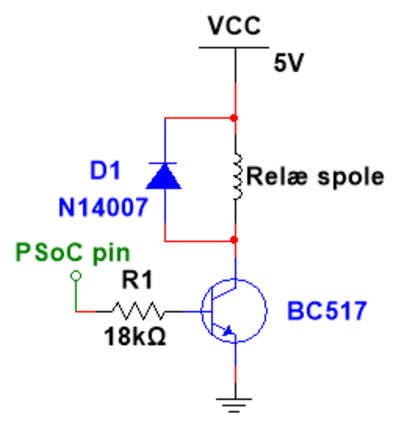
\includegraphics[width=0.3\textwidth]{filer/design/Billeder/BC517}}
\caption{BC517 opsætning}
\label{lab:BC517}
\raggedright
\end{figure} 

Når PSoC'ens pin til BC517 transistoren går høj (3,3 V), så skabes der forbindelse imellem collector og emitter på transistoren, herved er der 4 V over relæets spole og relæets kontaktsæt klikker herved. 

\subsection{Driver}

Driveren der skal håndtere Sprinkler-pumpe systemet, skal kunne aktivere/deaktivere det forudbestemte sprinklerrelæ. Metoden modtager en adresse parameter samt en on/off parameter. Herefter sætter metoden en af den forudbestemte pin på Enheden høj/lav (3.3 V / 0 V). Herefter sørger relæstyringen og 230 V / 5 V relæet for hhv. tænde/slukke for sprinkleren. 


\subsubsection*{Pseudokode}

\begin{lstlisting}[language=C]
void controlSprinkler(int address, bool on_off){
Manage Sprinkler address
Activate/deactivate corresponding Sprinkler
}
\end{lstlisting}





 